\documentclass[
    12pt,
    openright,
    oneside,
    a4paper,
    english,
    brazil,
    sumario=tradicional
]{abntex2}

% 1. Carrega as configurações e pacotes
\usepackage{lmodern}
\usepackage[T1]{fontenc}
\usepackage[utf8]{inputenc}

\usepackage{indentfirst}
\usepackage{microtype}
\usepackage{graphicx}
\usepackage{amsmath,amssymb}
\usepackage{booktabs}
\usepackage{longtable}
\usepackage{array}
\usepackage{multirow}
\usepackage{float}
\usepackage{caption}
\usepackage{subcaption}
\usepackage{xcolor}
\usepackage{url}
\usepackage{hyperref}

\usepackage[alf]{abntex2cite}
\usepackage{listings}

\definecolor{codebg}{RGB}{248,248,248}
\definecolor{codekw}{RGB}{0,102,204}
\definecolor{codecm}{RGB}{0,128,0}
\definecolor{codestr}{RGB}{163,21,21}

\lstdefinestyle{base}{
    backgroundcolor=\color{codebg},
    basicstyle=\ttfamily\footnotesize,
    breaklines=true,
    numbers=left,
    numberstyle=\tiny\color{gray},
    numbersep=8pt,
    frame=single,
    rulecolor=\color{gray!40},
    showstringspaces=false,
    tabsize=4,
    captionpos=b
}

\lstdefinestyle{cstyle}{
    style=base,
    language=C,
    commentstyle=\color{codecm}\itshape,
    keywordstyle=\color{codekw}\bfseries,
    stringstyle=\color{codestr}
}

\lstdefinestyle{x86}{
    style=base,
    language=[x86masm]Assembler,
    commentstyle=\color{codecm}\itshape,
    keywordstyle=\color{codekw}\bfseries
}

\lstdefinelanguage{ARMAssembly}{
    morekeywords={mov,add,sub,mul,ldr,str,ldp,stp,b,bl,ret,beq,bne,cbz,cbnz,cmp,adrp,adr,lsl,lsr,asr},
    sensitive=false,
    morecomment=[l]{//},
    morecomment=[s]{/*}{*/},
    morestring=[b]"
}

\lstdefinestyle{arm}{
    style=base,
    language=ARMAssembly,
    commentstyle=\color{codecm}\itshape,
    keywordstyle=\color{codekw}\bfseries,
    stringstyle=\color{codestr}
}

\lstdefinelanguage{RISCVAssembly}{
    morekeywords={lw,sw,add,sub,and,or,xor,beq,bne,blt,bge,jal,jalr,li,la,mv,ret,lui,auipc,slli,srli},
    sensitive=false,
    morecomment=[l]{\#},
    morestring=[b]"
}

\lstdefinestyle{riscv}{
    style=base,
    language=RISCVAssembly,
    commentstyle=\color{codecm}\itshape,
    keywordstyle=\color{codekw}\bfseries,
    stringstyle=\color{codestr}
}

\renewcommand{\lstlistingname}{Código}
\renewcommand{\lstlistlistingname}{Lista de códigos}
\renewcommand{\figurename}{Figura}
\renewcommand{\tablename}{Tabela}

\hypersetup{
    colorlinks=true,
    linkcolor=black,
    citecolor=black,
    urlcolor=blue,
    pdftitle={Arquiteturas RISC vs. CISC: características, aplicações e estudo de caso},
    pdfauthor={Arthur Martins Fonseca Dias; Arthur Freitas Araújo; Caio Seabra de Queiroz; Marina Souza Ramos}
}

\usepackage{titlesec}

\titleformat{\section}
{\normalfont\bfseries\raggedright}
{\thesection}
{1em}
{}

\titleformat{\subsection}
{\normalfont\bfseries\raggedright}
{\thesubsection}
{1em}
{}

\titleformat{\subsubsection}
{\normalfont\raggedright}
{\thesubsubsection}
{1em}
{}

\titlespacing*{\section}{0pt}{3.5ex plus 1ex minus .2ex}{2.3ex plus .2ex}
\titlespacing*{\subsection}{0pt}{3.25ex plus 1ex minus .2ex}{1.5ex plus .2ex}
\titlespacing*{\subsubsection}{0pt}{3.25ex plus 1ex minus .2ex}{1.5ex plus .2ex}

% ---------- Comandos personalizados para os dados do trabalho ----------
\providecommand{\curso}[1]{\def\imprimircurso{#1}}
\providecommand{\imprimircurso}{}
\providecommand{\disciplina}[1]{\def\imprimirdisciplina{#1}}
\providecommand{\imprimirdisciplina}{}
\providecommand{\professor}[1]{\def\imprimirprofessor{#1}}
\providecommand{\imprimirprofessor}{}
\usepackage{tikz}
\usetikzlibrary{shapes.geometric, arrows.meta, positioning, chains}

% 2. Define os dados do trabalho (isso vai preencher a capa automaticamente)
\titulo{Arquiteturas RISC vs.\ CISC: características, aplicações e estudo de caso}
\autor{Arthur Freitas Araújo \\ Arthur Martins Fonseca Dias \\ Caio Seabra de Queiroz \\ Marina Souza Ramos}
\local{Brasília -- DF}
\data{2026}
\instituicao{Universidade Católica de Brasília}
\curso{Ciência da Computação}
\disciplina{Arquitetura de Computadores}
\professor{Weldes Lima Oliveira}

\begin{document}

% --- Pré-textuais ---
\begin{capa}
    \centering

    % Instituição e Curso
    {\ABNTEXchapterfont\large\imprimirinstituicao\par}
    \vspace{0.5cm}
    {\ABNTEXchapterfont\large\imprimircurso\par}

    \vspace*{3cm}

    % Autores
    {\ABNTEXchapterfont\large\imprimirautor\par}

    \vspace*{2cm}

    % Título
    {\ABNTEXchapterfont\bfseries\Large\imprimirtitulo\par}

    \vfill

    % Texto de apresentação alinhado à direita
    \begin{flushright}
        \begin{minipage}{0.6\textwidth}
            \SingleSpacing
            Relatório técnico-acadêmico apresentado à \imprimirinstituicao, como parte dos requisitos avaliativos da unidade curricular de \imprimirdisciplina. \\
            Professor: \imprimirprofessor.
        \end{minipage}
    \end{flushright}

    \vfill

    % Local e Data
    {\large\imprimirlocal\par}
    {\large\imprimirdata\par}

\end{capa} % Apenas a capa unificada

\pdfbookmark[0]{\contentsname}{toc}
\tableofcontents*
\cleardoublepage

% --- Textuais (O Tema 5 em si) ---
\textual

\chapter{Introdução}
\label{cap:introducao}

\section{Contextualização}
O conjunto de instruções (ISA, \textit{Instruction Set Architecture}) é a interface entre o software e o hardware. Ele define as instruções que o processador executa, os tipos de operandos, os modos de endereçamento e os registradores acessíveis ao programador \cite{stallings2017}. Duas filosofias de projeto de ISA se consolidaram: RISC (\textit{Reduced Instruction Set Computer}) e CISC (\textit{Complex Instruction Set Computer}).

A filosofia RISC prioriza instruções simples e regulares, com o acesso à memória separado das operações aritméticas \cite{stallings2017}. A filosofia CISC admite instruções mais complexas, de formato variável, que podem operar diretamente sobre a memória \cite{silva2024}. Hoje a fronteira entre as duas é menos nítida: os processadores da linha x86 aceitam o conjunto de instruções CISC, mas o traduzem, em tempo de execução, para operações internas mais simples \cite{silva2024}.

\section{Importância para o desempenho}
O tempo de execução de um programa depende do número de instruções, dos ciclos gastos por instrução e da duração do ciclo de relógio (Equação~\ref{eq:tp}). As duas filosofias atuam sobre esses fatores de modos diferentes. Instruções complexas tendem a reduzir o número de instruções do programa, enquanto instruções simples e regulares facilitam a decodificação e o uso de \textit{pipeline} \cite{silva2024}.

Por isso, entender RISC e CISC ajuda a explicar o desempenho, o consumo de energia e as escolhas do compilador. Para quem desenvolve software, mostra também por que o mesmo código em C gera sequências de instruções diferentes em cada arquitetura.

\section{Objetivos}
\subsection{Objetivo geral}
Comparar as arquiteturas RISC e CISC, analisando suas características e aplicações, por meio de um estudo de caso e da análise do Assembly gerado a partir de um mesmo código em C.

\subsection{Objetivos específicos}
\begin{itemize}
  \item Apresentar os conceitos de ISA, RISC e CISC, a densidade de código, o \textit{pipeline} e a convergência entre as duas filosofias.
  \item Compilar o mesmo código em C para x86-64 e ARM64 no Compiler Explorer, com os níveis de otimização \texttt{-O0} e \texttt{-O2}, e comparar o Assembly gerado.
  \item Discutir os resultados da análise estática e suas limitações.
  \item Relacionar as diferenças entre as arquiteturas a cenários de uso em servidores e dispositivos móveis.
\end{itemize}

\section{Organização do trabalho}
O Capítulo~\ref{cap:fundamentacao} apresenta a fundamentação teórica. O Capítulo~\ref{cap:diagramas} traz os diagramas da arquitetura. O Capítulo~\ref{cap:metodologia} descreve a prova de conceito, com o código, o Assembly gerado e as métricas. O Capítulo~\ref{cap:discussao} discute os resultados e suas limitações. O Capítulo~\ref{cap:conclusao} reúne as conclusões.

\chapter{Fundamentação teórica}
\label{cap:fundamentacao}

\section{Arquitetura de conjunto de instruções (ISA)}
A ISA (Instruction Set Architecture) é a interface que separa o hardware do software. Ela define o formato das instruções (opcode e operandos), os modos de endereçamento, os registradores visíveis ao programador e o modelo de memória. É a ISA que garante que um mesmo código compilado possa rodar em processadores de diferentes fabricantes, desde que compartilhem a mesma arquitetura \cite{stallings2017}.

\section{Filosofia RISC}
A filosofia RISC (\textit{Reduced Instruction Set Computer}) baseia-se na simplicidade. Seus princípios incluem: instruções de tamanho fixo, poucos formatos de instrução e a separação estrita entre operações aritméticas e acessos à memória (arquitetura \textit{load/store}). Apenas as instruções de carga e armazenamento acessam a memória; o resto opera apenas sobre registradores. Isso facilita a implementação de \textit{pipelines} profundos e decodificadores mais simples e rápidos \cite{stallings2017}.

\section{Filosofia CISC}
\subsection{Arquitetura memória-memória}
Os processadores com arquitetura memória-memória possuem instruções aritméticas e lógicas onde todos os operandos são referenciados explicitamente. Ou seja, essas instruções possuem um total de três operandos, que podem estar localizados na memória. Apesar de, em grande parte dos casos, ainda ser necessário fazer uso de registradores, as instruções aritméticas e lógicas desses processadores têm a capacidade de referenciar todas as variáveis diretamente na memória \cite{silva2024}.

Normalmente, o código gerado pelos compiladores para essas máquinas é bastante eficiente, com um número bem menor de instruções de máquina. Em contrapartida, resultam em arquiteturas com implementação bastante complexa e sem possibilidade do uso de técnicas de otimização da execução das instruções, como o \textit{pipeline}. Como consequência, têm baixo desempenho quando comparadas com outras arquiteturas que adotaram soluções mais modernas, como os processadores RISC. Esse tipo de arquitetura é característico dos processadores CISC. Um exemplo de computador desse tipo é o VAX-11/780, um processador bastante comercializado nas décadas de 1970 e 1980 \cite{silva2024}.

\subsection{Arquitetura registrador-memória}
Os processadores com arquitetura registrador-memória normalmente possuem instruções aritméticas e lógicas com dois operandos, sendo que um deles está em memória e o outro em registrador. O resultado da operação é escrito automaticamente no mesmo registrador. Os exemplos clássicos desse tipo de arquitetura são o IBM 360 e os processadores da linha Intel x86. Em sua maioria, também são consideradas arquiteturas do tipo CISC, sendo que os processadores da linha x86, modernamente, implementam um tradutor que, em tempo de execução, faz a tradução de instruções x86 convencionais para instruções de um processador RISC implementado internamente \cite{silva2024}.

\begin{lstlisting}[caption={Exemplo de sequência em arquitetura registrador-memória (soma de A e B armazenada em C)}, label={lst:pseudo}]
LOAD R1, A
ADD R1, B
STORE C, R1
\end{lstlisting}

\subsection{Características da arquitetura CISC}
Uma outra maneira de melhorar o desempenho é diminuir o número total de instruções ($N_i$) gastas para traduzir um programa da linguagem de alto nível para a linguagem de máquina. Assim, instruções cada vez mais complexas eram implementadas no conjunto de instruções do processador. Essas instruções podiam realizar de uma só vez várias operações complexas, acessando o maior número possível de operandos de uma única vez, com vários e diversos modos de endereçamento possíveis.

Essa aproximação foi adotada pelas arquiteturas CISC (\textit{Complex Instruction Set Computer}), presentes nas primeiras arquiteturas de processadores, incluindo as dos primeiros microprocessadores, até o início da década de 1980. Exemplos de arquitetura CISC são os antigos processadores x86 da Intel e o VAX-11/780, entre outros computadores clássicos.

Resumindo, as arquiteturas CISC são caracterizadas por instruções complexas, que frequentemente demandam um grande número e variável de ciclos de relógio para serem executadas. Essas instruções possuem formatos variáveis e diversos modos de endereçamento dos operandos. Vários tipos de instruções podem acessar os seus operandos diretamente na memória. Como resultado, há uma dificuldade grande para o uso de técnicas como \textit{pipeline} na implementação desses processadores. A taxa média de execução das instruções por ciclo tende a ser bastante superior a 1 ciclo por instrução (CPI) e a unidade de controle desses processadores é, em geral, microprogramada. Como grande vantagem, os compiladores podem gerar códigos compactos, com um reduzido número de instruções \cite{silva2024}.

\section{Densidade de código e complexidade de decodificação}
Um dos objetivos da arquitetura de um processador é permitir a execução dos programas o mais rapidamente possível. Há várias técnicas que são empregadas para isso, mas, de uma forma simplificada, o tempo de execução de um programa pode ser definido pela seguinte equação:

\begin{equation}
    T_p = C_i \times T_c \times N_i
    \label{eq:tp}
\end{equation}

Em que:
\begin{itemize}
    \item $T_p$ é o tempo de execução do programa;
    \item $C_i$ são os ciclos gastos em média por instrução;
    \item $T_c$ é o tempo de duração de um ciclo;
    \item $N_i$ é o número de instruções do programa.
\end{itemize}

O $C_i$ também é conhecido como CPI (Ciclos por Instrução) e define o número médio de ciclos gastos por cada instrução. É um valor que varia de acordo com cada programa, por exemplo, se possui mais instruções inteiras ou de ponto flutuante, além do tipo da arquitetura do processador. O CPI é obtido dividindo-se o número total de ciclos de relógio gastos para executar um programa pelo total de instruções executadas. O seu inverso é o IPC (Instruções por Ciclo), mais usado modernamente nas arquiteturas superescalares, para indicar o número de instruções, normalmente maior do que um, que podem ser executadas a cada ciclo de relógio do processador. O tempo de ciclo ($T_c$) é o inverso da frequência do relógio $f$, segundo a fórmula:

\begin{equation}
    T_c = \frac{1}{f}
    \label{eq:tc}
\end{equation}

Por exemplo, se a frequência do relógio for 100 MHz ($100 \times 10^{6}$ Hz), o tempo de ciclo será de 10 ns ($10 \times 10^{-9}$ s). Logo, quanto maior for a frequência do relógio, menor será o tempo de ciclo e menor será o tempo total de execução dos programas.

Em contrapartida, nas arquiteturas CISC o número de ciclos para executar cada instrução é muito maior, e um hardware mais complexo resultava em frequências de relógio menores, em virtude do longo tempo necessário para a decodificação das instruções \cite{silva2024}.

\section{Consumo de energia e contagem de transistores}
Durante algum tempo os projetistas buscaram reduzir o tempo de execução dos programas aumentando ao máximo a frequência do relógio do processador, a partir de diversas técnicas de projeto, por exemplo, o \textit{superpipelining}. Entretanto, essa abordagem tem um limite em função do atraso mínimo dos componentes do processador, assim como da potência máxima que podia ser dissipada pelo conjunto encapsulamento e dissipador \cite{silva2024}.

Historicamente, acreditava-se que processadores CISC, por serem mais complexos, consumiriam mais energia. No entanto, em processadores modernos, o consumo está mais atrelado à tensão de operação, à frequência e à eficiência do \textit{pipeline} do que à classificação RISC ou CISC. Decodificadores complexos gastam mais energia, mas o uso extensivo de caches e a execução fora de ordem (\textit{out-of-order}) também elevam o consumo em ambas as arquiteturas.

\section{Pipeline}
O \textit{pipeline} é uma técnica de implementação de processadores que permite a sobreposição temporal das diversas fases de execução das instruções. Essa técnica aumenta o número de instruções executadas simultaneamente e a taxa de instruções iniciadas e terminadas por unidade de tempo. Contudo, o \textit{pipeline} não reduz o tempo gasto para completar cada instrução individualmente, podendo até mesmo aumentá-lo em alguns casos \cite{silva2024}.

\section{Convergência moderna}
Atualmente, os processadores da Intel são uma arquitetura híbrida, externamente compatíveis com o código da arquitetura x86, mas com as instruções traduzidas, em tempo de execução, para as instruções RISC da arquitetura interna, que efetivamente executa os programas \cite[p.~74]{silva2024}.

Arquiteturas RISC modernas, como o ARM, também adicionaram instruções complexas para processamento de mídia (como NEON e SVE), mostrando que a fronteira entre as filosofias se tornou tênue \cite{arm2024}.
\chapter{Mapeamento e diagrama arquitetural}
\label{cap:diagramas}

\section{Fluxo de execução de instruções}
O ciclo básico de execução de qualquer processador é composto por três etapas fundamentais: busca (\textit{fetch}), decodificação (\textit{decode}) e execução (\textit{execute}). O contador de programa (PC) armazena o endereço da próxima instrução a ser executada. A unidade de controle busca essa instrução na memória e a decodifica para saber qual operação realizar. Em seguida, a ULA (Unidade Lógica e Aritmética) executa a operação, e o resultado pode ser armazenado em um registrador ou na memória.

\begin{figure}[htbp]
    \centering
    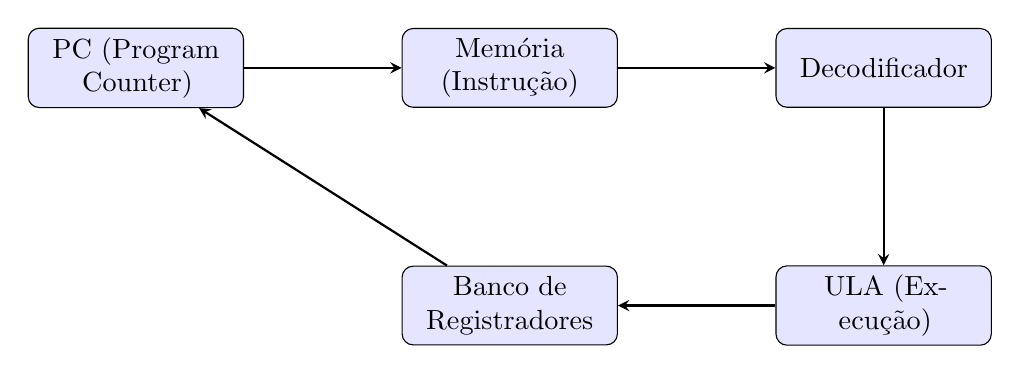
\begin{tikzpicture}[
        node distance=2cm,
        box/.style={rectangle, draw, fill=blue!10, text width=2.5cm, text centered, minimum height=1cm, rounded corners},
        arrow/.style={thick,->,>=stealth}
    ]
        \node (pc) [box] {PC (Program Counter)};
        \node (mem) [box, right=of pc] {Memória (Instrução)};
        \node (dec) [box, right=of mem] {Decodificador};
        \node (ula) [box, below=of dec] {ULA (Execução)};
        \node (reg) [box, left=of ula] {Banco de Registradores};

        \draw [arrow] (pc) -- (mem);
        \draw [arrow] (mem) -- (dec);
        \draw [arrow] (dec) -- (ula);
        \draw [arrow] (ula) -- (reg);
        \draw [arrow] (reg) -- (pc);
    \end{tikzpicture}
    \caption{Ciclo de busca, decodificação e execução}
    \label{fig:ciclo}
\end{figure}

\section{Fluxo de instrução em RISC e em CISC}
Em arquiteturas RISC, a instrução lida da memória é decodificada diretamente pelo hardware, pois possui formato fixo e regular, sendo executada logo em seguida. Em arquiteturas CISC, especialmente no x86, a instrução complexa lida da memória passa por um tradutor que a converte em micro-operações menores (que se parecem com instruções RISC). São essas micro-operações que efetivamente entram no pipeline de execução.

\section{Registradores das arquiteturas da PoC}
Para entender o Assembly gerado na prova de conceito, é preciso conhecer os registradores de cada arquitetura:
\begin{itemize}
    \item \textbf{x86-64:} Os registradores de uso geral têm 64 bits e incluem \texttt{rax}, \texttt{rbx}, \texttt{rcx}, \texttt{rdx}, \texttt{rsi}, \texttt{rdi}, \texttt{rbp} e \texttt{rsp} (este último o ponteiro de pilha). O \texttt{rax} é frequentemente usado para acumuladores e retorno de funções.
    \item \textbf{ARM64:} Possui 31 registradores de uso geral, nomeados de \texttt{x0} a \texttt{x30} (64 bits), além do \texttt{sp} (stack pointer) e \texttt{pc} (program counter). Quando o processador precisa operar com 32 bits, utiliza a visão \texttt{w0} a \texttt{w30} (ex: \texttt{w0} é a metade inferior de \texttt{x0}).
\end{itemize}

\section{Diagrama de pipeline comparativo}
O pipeline moderno é dividido em estágios (IF, ID, EX, MEM, WB). O RISC foi desenhado para preencher esses estágios com facilidade devido ao tamanho fixo das instruções, o que facilita a sobreposição. O CISC moderno também usa pipeline, mas necessita do estágio extra de tradução para micro-operações antes de entrar na execução.

\begin{figure}[htbp]
    \centering
    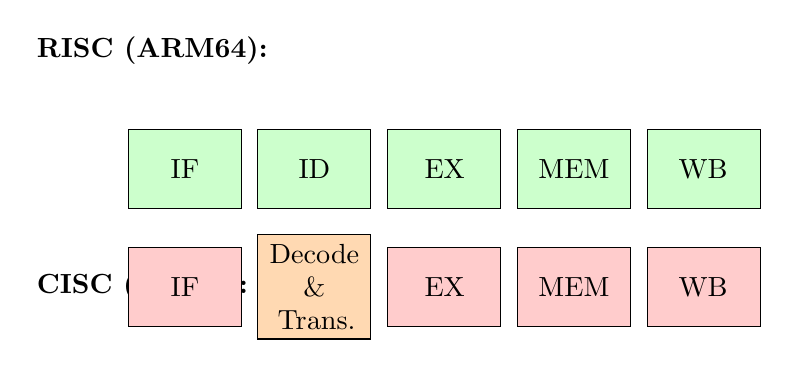
\begin{tikzpicture}[
        start chain=going right,
        node distance=0.2cm,
        stage/.style={rectangle, draw, fill=green!20, text width=1.2cm, text centered, minimum height=1cm},
        ciscstage/.style={rectangle, draw, fill=red!20, text width=1.2cm, text centered, minimum height=1cm}
    ]
        % RISC Pipeline
        \node[font=\bfseries, anchor=west] at (-2, 1.5) {RISC (ARM64):};
        \node[stage, on chain] {IF};
        \node[stage, on chain] {ID};
        \node[stage, on chain] {EX};
        \node[stage, on chain] {MEM};
        \node[stage, on chain] {WB};

        % CISC Pipeline
        \node[font=\bfseries, anchor=west] at (-2, -1.5) {CISC (x86-64):};
        \node[ciscstage] (fetch) at (0, -1.5) {IF};
        \node[ciscstage, right=0.2cm of fetch, fill=orange!30] (decode) {Decode \& Trans.};
        \node[ciscstage, right=0.2cm of decode] (exec) {EX};
        \node[ciscstage, right=0.2cm of exec] (mem) {MEM};
        \node[ciscstage, right=0.2cm of mem] (wb) {WB};
    \end{tikzpicture}
    \caption{Comparação de pipelines: RISC direto vs. CISC com tradução para micro-operações}
    \label{fig:pipeline}
\end{figure}
\chapter{Metodologia e desenvolvimento}
\label{cap:metodologia}

\section{Ambiente e ferramentas}
Utilizou-se o Compiler Explorer (Godbolt) \cite{godbolt} para compilar o mesmo código em C para duas arquiteturas. Os compiladores foram o \textit{x86-64 gcc 16.1} e o \textit{ARM64 GCC 16.1.0}, da mesma família e versão principal, para que a diferença observada venha da arquitetura e não do compilador. Foram usados os níveis de otimização \texttt{-O0} e \texttt{-O2}. O acesso à ferramenta ocorreu em 4 de novembro de 2026.

\section{Arquiteturas selecionadas}
Foram selecionadas a arquitetura x86-64, classificada como CISC, e a ARM64, classificada como RISC \cite[p.~23--28]{stallings2017}\cite[p.~31--36]{tanenbaum2013}. Em processadores modernos essa distinção é sutil, como discutido no Capítulo~\ref{cap:fundamentacao}.

\section{Código-fonte em C}
O trecho analisado soma os elementos positivos de um vetor. Ele reúne laço de repetição, condição, leitura da memória e acumulação em uma variável.

\lstinputlisting[style=cstyle, caption={Código em C da PoC}, label={lst:c}]{poc/c/soma_positivos.c}

\section{Assembly gerado}
\subsection{x86-64}
\lstinputlisting[style=x86, caption={Assembly x86-64, gcc 16.1, -O0}, label={lst:x86o0}]{poc/asm/x86-64_O0.s}
\lstinputlisting[style=x86, caption={Assembly x86-64, gcc 16.1, -O2}, label={lst:x86o2}]{poc/asm/x86-64_O2.s}

\subsection{ARM64}
\lstinputlisting[style=arm, caption={Assembly ARM64, gcc 16.1.0, -O0}, label={lst:armo0}]{poc/asm/arm64_O0.s}
\lstinputlisting[style=arm, caption={Assembly ARM64, gcc 16.1.0, -O2}, label={lst:armo2}]{poc/asm/arm64_O2.s}

\subsection{Comentários sobre as listagens}
\textbf{x86-64, \texttt{-O0}.} Todas as variáveis ficam na pilha, acessadas por endereços relativos a \texttt{rbp}. O prólogo \texttt{push rbp} e \texttt{mov rbp, rsp} monta o quadro de pilha. O teste do \texttt{for} vira \texttt{cmp} seguido de \texttt{jl .L4}, e o \texttt{if} vira \texttt{test} seguido de \texttt{jle .L3}, que salta sobre a soma quando o elemento não é positivo. A acumulação é feita por \texttt{add DWORD PTR [rbp-4], eax}, uma única instrução que lê e escreve a memória.

\textbf{ARM64, \texttt{-O0}.} O quadro de pilha é reservado por \texttt{sub sp, sp, \#32}. Apenas \texttt{ldr}, \texttt{ldrsw} e \texttt{str} acessam a memória; \texttt{add}, \texttt{lsl} e \texttt{cmp} operam sobre registradores. O endereço de \texttt{v[i]} é calculado por \texttt{lsl} e \texttt{add}. O \texttt{for} vira \texttt{cmp} e \texttt{blt .L4}, e o \texttt{if} vira \texttt{cmp} e \texttt{ble .L3}. A mesma acumulação exige três instruções: \texttt{ldr}, \texttt{add} e \texttt{str}.

\textbf{x86-64, \texttt{-O2}.} As variáveis passam para registradores e a pilha deixa de ser usada. O \texttt{if} não gera salto: \texttt{test eax, eax} e \texttt{cmovs eax, ecx} substituem o valor por zero quando ele é negativo. O laço percorre o vetor por ponteiro, com \texttt{add rdi, 4} e \texttt{cmp rdi, rsi} seguido de \texttt{jne .L4}. O único acesso à memória é \texttt{mov eax, DWORD PTR [rdi]}.

\textbf{ARM64, \texttt{-O2}.} A instrução \texttt{ldr w2, [x3], 4} carrega o elemento e avança o ponteiro em uma só operação (pós-incremento). O \texttt{if} também some como salto: \texttt{bic w2, w2, w2, asr \#31} zera os valores negativos. O laço fecha com \texttt{cmp x3, x1} e \texttt{bne .L4}.

\section{Passo a passo da PoC}
\begin{enumerate}
  \item Abrir o Compiler Explorer e escolher a linguagem C.
  \item Colar o código do Código~\ref{lst:c} no editor.
  \item Selecionar o compilador x86-64 gcc 16.1 e informar a opção \texttt{-O0}.
  \item Adicionar um segundo painel de compilação (\textit{Add new}) com o ARM64 GCC 16.1.0 e a mesma opção \texttt{-O0}.
  \item Copiar o Assembly de cada painel e salvar em arquivo.
  \item Repetir os passos 3 a 5 com a opção \texttt{-O2}.
  \item Registrar a tela de cada configuração (Figuras~\ref{fig:godbolt_o0} e \ref{fig:godbolt_o2}).
\end{enumerate}

\begin{figure}[htb]
  \caption{Compiler Explorer com x86-64 e ARM64, opção -O0}
  \label{fig:godbolt_o0}
  \centering
  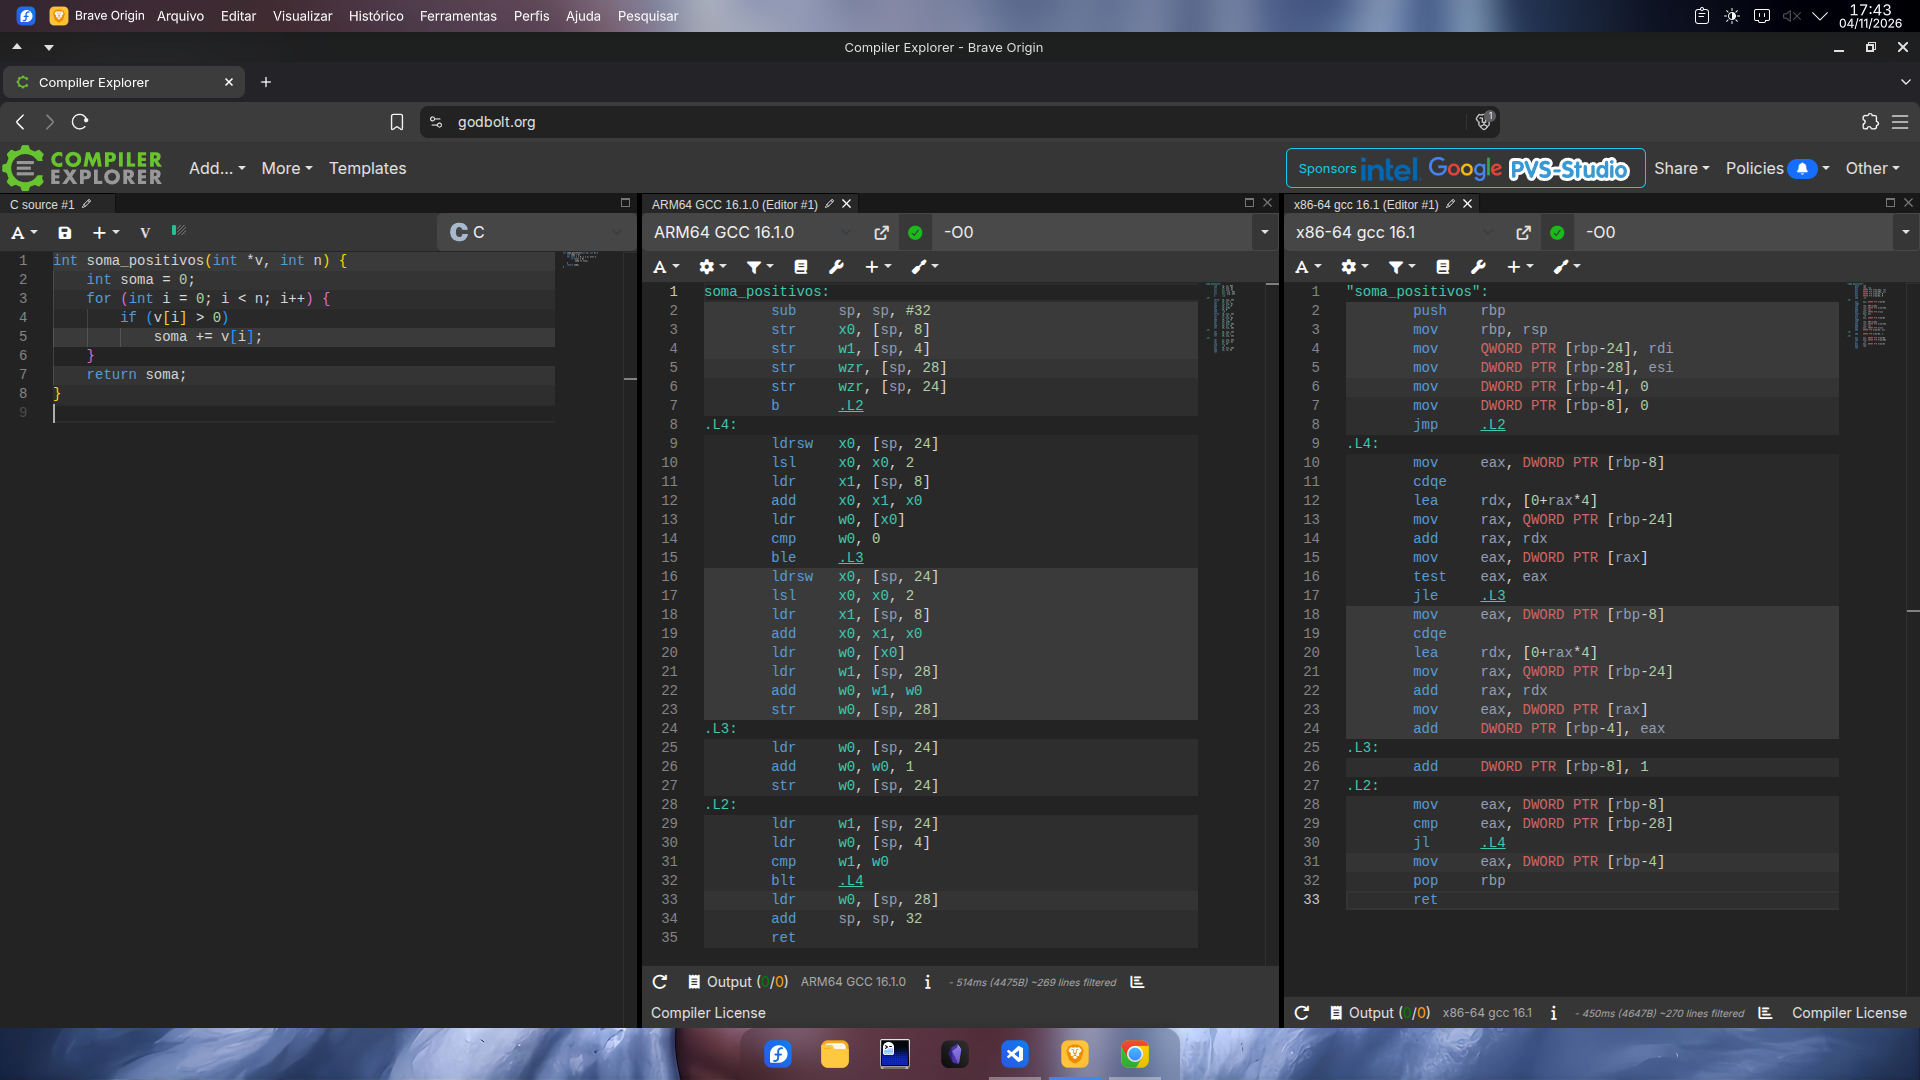
\includegraphics[width=\textwidth]{poc/capturas/godbolt_O0.png}
  \legend{Fonte: elaborado pelos autores no Compiler Explorer.}
\end{figure}

\begin{figure}[htb]
  \caption{Compiler Explorer com x86-64 e ARM64, opção -O2}
  \label{fig:godbolt_o2}
  \centering
  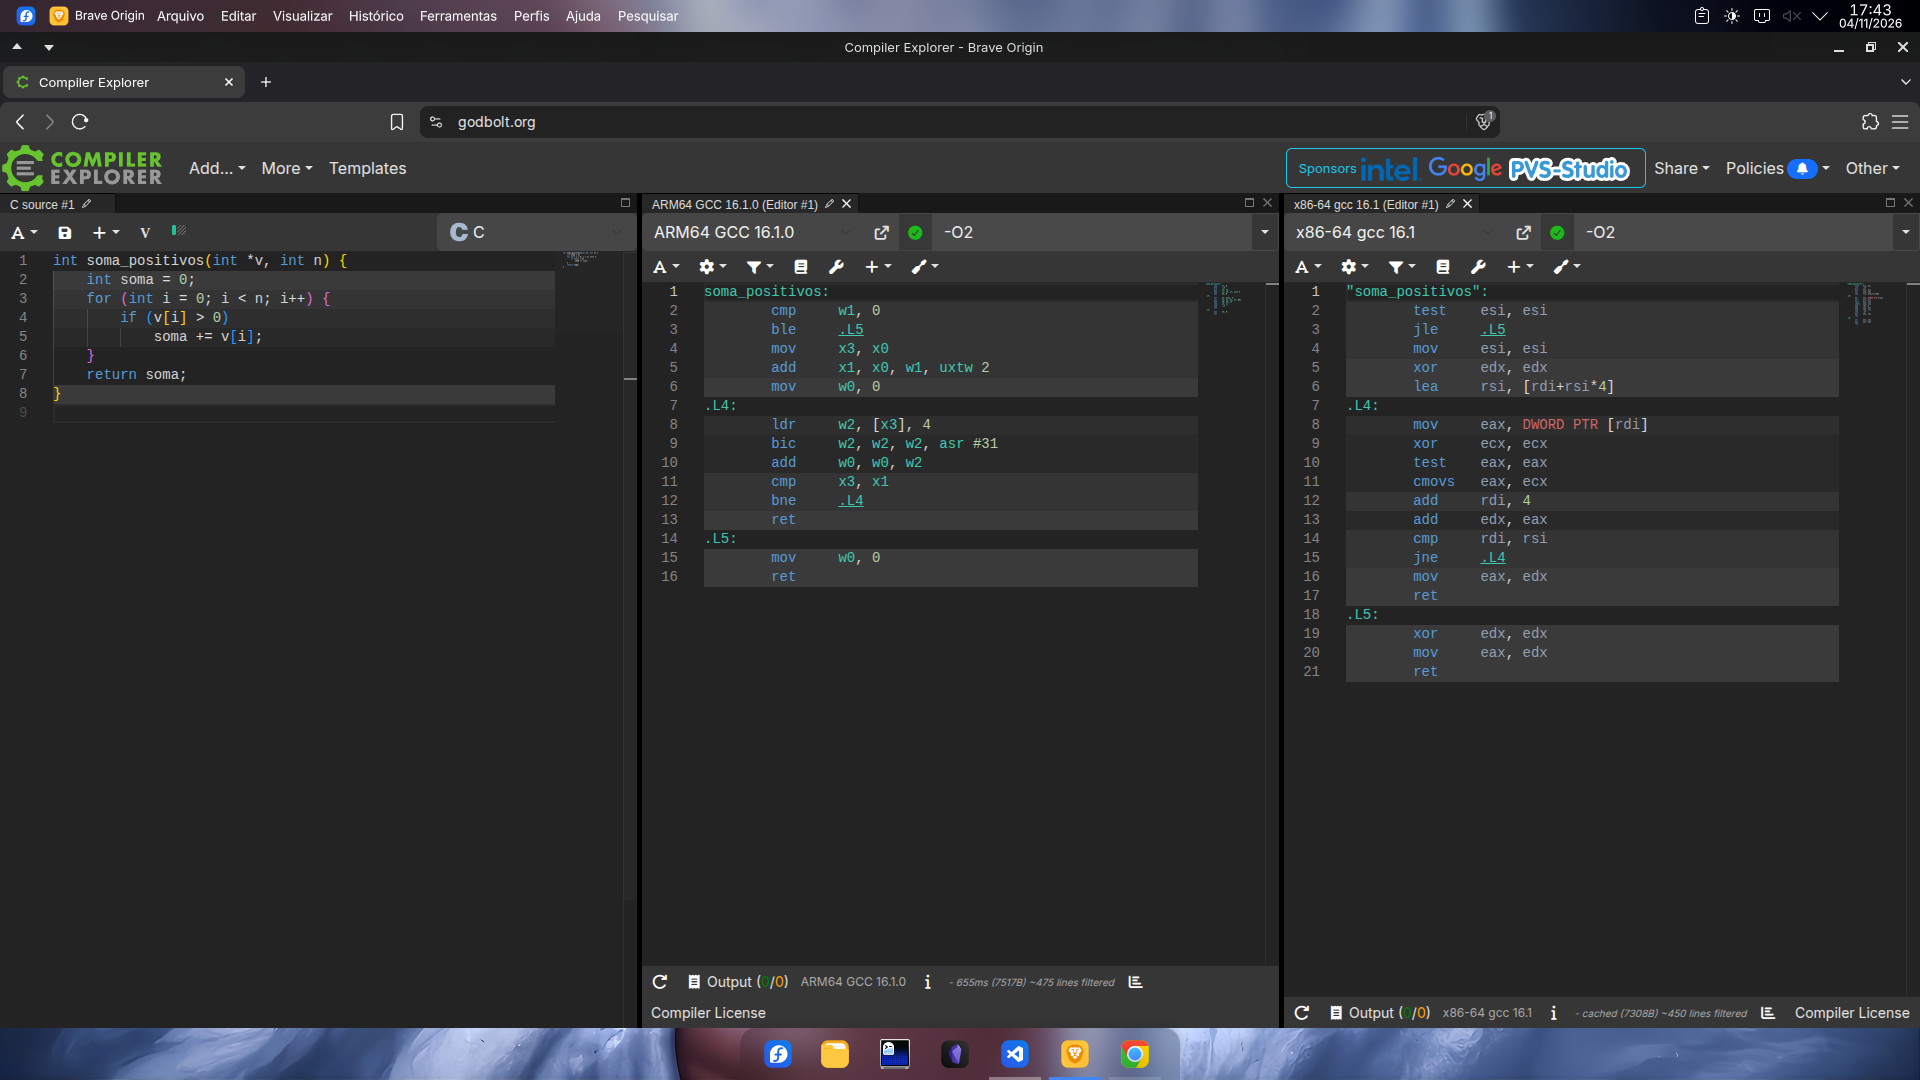
\includegraphics[width=\textwidth]{poc/capturas/godbolt_O2.png}
  \legend{Fonte: elaborado pelos autores no Compiler Explorer.}
\end{figure}

\section{Métricas coletadas}
Foram coletadas métricas estáticas, contadas sobre o texto do Assembly gerado:
\begin{itemize}
  \item \textbf{Instruções:} linhas de instrução, sem contar rótulos e o nome da função. O retorno é contado.
  \item \textbf{Saltos:} instruções de desvio condicional e incondicional. O retorno não é contado.
  \item \textbf{Acessos à memória:} em ARM64, as instruções de carga e armazenamento. Em x86-64, as instruções com operando de memória, exceto \texttt{lea}, que apenas calcula o endereço.
  \item \textbf{Registradores utilizados:} registradores de uso geral distintos, tratando as visões de 32 e 64 bits como um só registrador (por exemplo, \texttt{eax} e \texttt{rax}). Ponteiro de pilha (\texttt{sp}, \texttt{rsp}) e registrador zero (\texttt{wzr}) não são contados; o \texttt{rbp}, usado como base do quadro de pilha, é contado.
  \item \textbf{Bytes de código:} tamanho da função lido na saída binária do Compiler Explorer. Em ARM64, cada instrução ocupa 4 bytes; em x86-64, o tamanho varia. Em \texttt{-O2}, os bytes incluem 3 instruções \texttt{nop} de alinhamento em cada arquitetura, que não entram na contagem de instruções.
\end{itemize}
Os valores estão na Tabela~\ref{tab:comparacao}, no Capítulo~\ref{cap:discussao}.

\section{Limitação do método}
O Godbolt realiza análise estática. Ele mostra as instruções geradas, mas não executa o programa e não mede ciclos reais. Contagem de instruções não equivale a desempenho. Os resultados valem para este trecho de código e para as versões de compilador usadas.
\chapter{Discussão dos resultados}
\label{cap:discussao}

\section{Métricas obtidas}
\begin{table}[htb]
    \caption{Comparação estática do código gerado (gcc 16.1)}
    \label{tab:comparacao}
    \centering
    \begin{tabular}{lcccc}
        \toprule
                                 & \multicolumn{2}{c}{\texttt{-O0}} & \multicolumn{2}{c}{\texttt{-O2}}                  \\
        \cmidrule(lr){2-3} \cmidrule(lr){4-5}
        Métrica                  & x86-64                           & ARM64                            & x86-64 & ARM64 \\
        \midrule
        Instruções               & 29                               & 31                               & 18     & 13    \\
        Saltos                   & 3                                & 3                                & 2      & 2     \\
        Acessos à memória        & 15                               & 17                               & 1      & 1     \\
        Registradores utilizados & 5                                & 2                                & 5      & 4     \\
        Bytes de código          & 95                               & 124                              & 66     & 64    \\
        \bottomrule
    \end{tabular}
    \legend{Fonte: elaborado pelos autores com dados do Compiler Explorer. Em \texttt{-O2}, os bytes incluem 3 instruções \texttt{nop} de alinhamento em cada arquitetura, não contadas em ``Instruções''.}
\end{table}

\section{Análise da comparação}
Em \texttt{-O0}, o ARM64 executa 31 instruções contra 29 do x86-64, e ocupa mais bytes (124 contra 95). A largura fixa de 4 bytes do ARM64 contrasta com as instruções de tamanho variável do x86-64. Em \texttt{-O2}, o ARM64 usa 13 instruções contra 18, e os bytes quase empatam (64 contra 66). Nos dois níveis, a mudança de otimização altera mais a contagem do que a mudança de arquitetura.

\section{Do código em C ao hardware}
O laço \texttt{for} vira uma comparação seguida de salto condicional: \texttt{cmp} e \texttt{jl} no x86-64, \texttt{cmp} e \texttt{blt} no ARM64. Em \texttt{-O0}, a acumulação \texttt{soma += v[i]} mostra a diferença entre as filosofias. No x86-64, \texttt{add DWORD PTR [rbp-4], eax} lê e escreve a memória em uma instrução. No ARM64, são necessárias \texttt{ldr}, \texttt{add} e \texttt{str}, pois apenas carga e armazenamento acessam a memória. Em \texttt{-O2}, as variáveis passam para registradores e o \texttt{if} deixa de gerar salto: \texttt{cmovs} no x86-64 e \texttt{bic} no ARM64.

\section{Limitações do método}
O Godbolt fornece análise estática. Ele mostra as instruções geradas, mas não executa o programa e não mede ciclos reais, tempo de CPU, cache, previsão de saltos nem execução fora de ordem. Contagem de instruções e de bytes não equivale a desempenho. Os resultados valem para este trecho de código e para o gcc 16.1.

\section{Limitações físicas}
O consumo de energia e a dissipação de calor limitam o aumento da frequência de operação dos processadores. Por isso, o ganho de desempenho passou a depender de paralelismo e de eficiência por instrução \cite[p.~24--28]{patterson2017}. A contagem de transistores também tem custo de área e de energia, e decodificadores de instruções irregulares ocupam mais recursos que decodificadores de instruções regulares \cite[p.~408--410, 560--562]{stallings2017}.

Atribuir diferenças de consumo apenas à classificação RISC ou CISC é uma simplificação, pois cache, pipeline e processo de fabricação também influenciam o resultado. Na PoC, o ARM64 usa instruções de largura fixa de 4 bytes, enquanto o x86-64 usa instruções de tamanho variável. Esse contraste de formato é o que torna a decodificação do x86-64 mais complexa \cite[p.~289--292]{tanenbaum2013}. A PoC, porém, é estática: não mede consumo, área nem frequência.

\section{Estudo de caso: servidores e dispositivos móveis}
Para o mesmo trecho em C, a PoC mostra o que cada ISA exige do compilador e do hardware. O x86-64 permite operar diretamente sobre a memória, como em \texttt{add DWORD PTR [rbp-4], eax}, e tem instruções de tamanho variável \cite{intel2024}. O ARM64 separa o acesso à memória da aritmética (\texttt{ldr}, \texttt{add}, \texttt{str}) e tem instruções de tamanho fixo \cite{arm2024}. Esses traços orientam o uso de cada arquitetura, mas não bastam para afirmar qual é melhor em servidores ou em dispositivos móveis, pois isso depende de energia, desempenho medido e compatibilidade de software.

No mercado, as duas arquiteturas coexistem. Em servidores x86-64, a Intel e a AMD dividem a receita de CPUs para servidores: no primeiro trimestre de 2026, a Intel ficou com 53,8\% e a AMD com 46,2\% \cite{exame2026}. Em nuvem, a Amazon projetou processadores ARM próprios, os Graviton, oferecidos como máquinas virtuais na AWS \cite{register2018}. Em computadores pessoais, a Apple anunciou em 2020 a troca dos processadores Intel por chips próprios de arquitetura ARM, a mesma usada em iPhones e iPads \cite{canaltech2020}.

\section{Impacto no desenvolvimento de software de alto desempenho}
A ISA aparece para o programador por meio do compilador. O mesmo código C gerou sequências diferentes em x86-64 e ARM64, e o programa precisa ser recompilado para cada arquitetura \cite{godbolt}. Na PoC, a troca de \texttt{-O0} para \texttt{-O2} alterou a contagem de instruções mais do que a troca de arquitetura (Tabela~\ref{tab:comparacao}). Para quem escreve software de alto desempenho, isso significa que as opções do compilador e a escolha de algoritmos pesam tanto quanto a ISA.

Os efeitos de cache, previsão de saltos e execução fora de ordem não foram medidos neste trabalho. A análise de um programa real exige medição de tempo e de contadores de hardware, além do Assembly. Detalhes de cada instrução devem ser conferidos nos manuais das arquiteturas \cite{intel2024,arm2024}.
\chapter{Conclusão}
\label{cap:conclusao}

\section{Síntese do aprendizado}
Este trabalho comparou as arquiteturas RISC e CISC, utilizando a análise estática do Assembly gerado pelo Compiler Explorer como prova de conceito. Os objetivos foram atingidos ao demonstrar que, embora o x86-64 (CISC) tenha gerado menos instruções em nível de otimização zero (-O0), ele utiliza instruções de tamanho variável que tornam a decodificação mais complexa. Por outro lado, o ARM64 (RISC) gerou mais instruções, porém com largura fixa e separação clara entre operações de memória (load/store) e de registradores.

\section{Lições aprendidas}
A principal lição é que a divisão entre RISC e CISC não é mais uma fronteira rígida. Os processadores modernos convergiram: o x86-64 traduz instruções complexas em micro-operações internas (tornando-se RISC por dentro), enquanto o ARM64 adiciona extensões complexas (como vetorização) para ganhar desempenho. Além disso, a PoC mostrou que o nível de otimização do compilador (de -O0 para -O2) altera drasticamente o código gerado, reduzindo a contagem de instruções e muitas vezes superando o impacto da própria mudança de arquitetura. O uso de instruções como \texttt{cmovs} e \texttt{bic} elimina saltos condicionais, otimizando o pipeline.

\section{Implicações práticas}
Para o desenvolvimento de software de alto desempenho, entender a arquitetura é fundamental para escolher a melhor linguagem, as flags de compilação corretas e as estruturas de dados adequadas. O programador precisa saber que o mesmo código em C terá um comportamento de hardware diferente em um servidor x86 e em um dispositivo móvel ARM, e que o compilador fará otimizações agressivas quando solicitado. Compreender como o laço \texttt{for} se transforma em saltos e como a memória é acessada permite escrever códigos que exploram melhor a localidade e o poder de processamento dos processadores modernos.

% --- Pós-textuais ---
\postextual
\nocite{patterson2017,stallings2017,tanenbaum2013,monteiro2007,weber2012,intel2024,arm2024,riscv2019,godbolt}
\bibliography{referencias}


\end{document}